\section{Daredevil y su astigmatismo (1 pt)}

Daredevil está muy preocupado con la situación de la salud en el país, ya que le dijeron que mientras más ciego esté,  más fila le toca hacer para reclamar los medicamentos para la ceguera. Dado que él no está seguro del porcentaje de miopía y astigmatismo que presenta, decide pedir una cita con el oftanmólogo. Sin embargo, se la dieron para septiembre. El Punisher le dice entonces que la única forma de lograr la cita rápido, es armando un "mierdero" en la EPS, pero éste se rehúsa a armarlo; en su lugar, investiga en ChatGPT cuál sería la fórmula para calcular el porcentaje de miopía y astigmatismo de una persona. La IA le arroja la siguiente expresión:

\[
f(x) \;=\; \frac{A\times 10^{-2}}{8} \,\cos\bigl(x \;-\; A\times 10^{-3}\bigr) \;-\; x,
\]
siendo \(x \times 100\%\) el porcentaje de miopía y astigmatismo de la persona, y \(A\) corresponde a 510. El problema se reduce a resolver \(f(x) = 0\).

\subsection{Ayude al Diablo}

Ayude  al Diablo a calcular su porcentaje de ceguera, usando $510$, y el
método de punto fijo con una tolerancia de 6 cifras significativas, y una
condición inicial $x_0 = 0$. Note que $g(x) = f(x) - x$.
Dé una respuesta al Diablo, y entregue la tabla solución en el formato visto en clase.

Sea la función dada:
\[
f(x) \;=\; \frac{A\times10^{-2}}{8}\,\cos\bigl(x - A\times10^{-3}\bigr)\;-\;x
\quad\text{con}\quad A=510.
\]
La raíz de la ecuación \(f(x)=0\) proporciona \(x \times 100\%\) como porcentaje de miopía y astigmatismo.

\subsection{Aplicación del método de punto fijo}

Para \(A = 510\),
\[
A\times 10^{-2} \;=\; 5.1,
\quad
\frac{5.1}{8} \;=\; 0.6375,
\quad
A\times 10^{-3} \;=\; 0.510.
\]
Por lo tanto, la función de iteración es
\[
g(x) \;=\; 0.6375 \,\cos\bigl(x \;-\; 0.510\bigr).
\]
Con \(x_0 = 0\) y tolerancia \(10^{-6}\), se ejecuta:
\[
x_{n+1} \;=\; g(x_n) \;=\; 0.6375 \,\cos\bigl(x_n - 0.510\bigr).
\]

\subsection{Tabla de iteraciones}

A continuación, se muestra la tabla generada (formato \texttt{long} en \textsc{Matlab}). En cada paso se listan: el índice \(n\), la aproximación \(x_n\), el valor \(f(x_n)\) y el error.

\[
\begin{array}{c|c|c|c}
\toprule
\textbf{n} 
& x_n 
& f(x_n)\;=\;\dfrac{A\times10^{-2}}{8}\cos(x_n - A\times 10^{-3}) - x_n
& Error \\
\midrule
0 & 0.000000000000000 & 0.556374623624166 & 1.000001000000000 \\[6pt]
1 & 0.556374623624166 & 0.080439993649312 & 0.556374623624166 \\[6pt]
2 & 0.636814617273478 & -0.004433871777047 & 0.080439993649312 \\[6pt]
3 & 0.632380745496431 & 0.000351276126239 & 0.004433871777047 \\[6pt]
4 & 0.632732021622670 & -0.000027376443341 & 0.000351276126239 \\[6pt]
5 & 0.632704645179329 & 0.000002136367937 & 0.000027376443341 \\[6pt]
6 & 0.632706781547266 & -0.000000166698095 & 0.000002136367937 \\[6pt]
7 & 0.632706614849171 & 0.000000013007346 & 0.000000166698095 \\
\bottomrule
\end{array}
\]

En la iteración \(n=7\), se logra un error menor que \(10^{-6}\). Por tanto, la aproximación final con 6 cifras significativas es

\[
x \;\approx\; 0.632707.
\]

\subsection{Resultado Final}

Puesto que la fracción \(x\) multiplicada por 100\% indica el porcentaje de miopía y astigmatismo, se concluye:
\[
\boxed{
\text{Porcentaje de ceguera} 
\;\approx\; 63.2707\%.
}
\]

Con la presición solicitada ($63.2707\%$) parece que el Diablo a duras penas va
a poder ver la fila en la EPS.

\section{Análisis Gráfico (1 pt)}

El Diablo no creía en este método, sin embargo ha encontrado una solución con
el mismo. Explique gráficamente porque se encontró una solución, verificando si
la función $g(x)$ cumple los criterios del teorema de punto fijo en el intervalo
$[0, 2]$, para ser una buena función. (Verifique los tres criterios). Entregue su procedimiento y respuesta. 

\subsection{Gráfico de $f(x)$ y $g(x)$}
\begin{figure}[H]
    \centering
    \begin{subfigure}[b]{\textwidth}
        \centering
        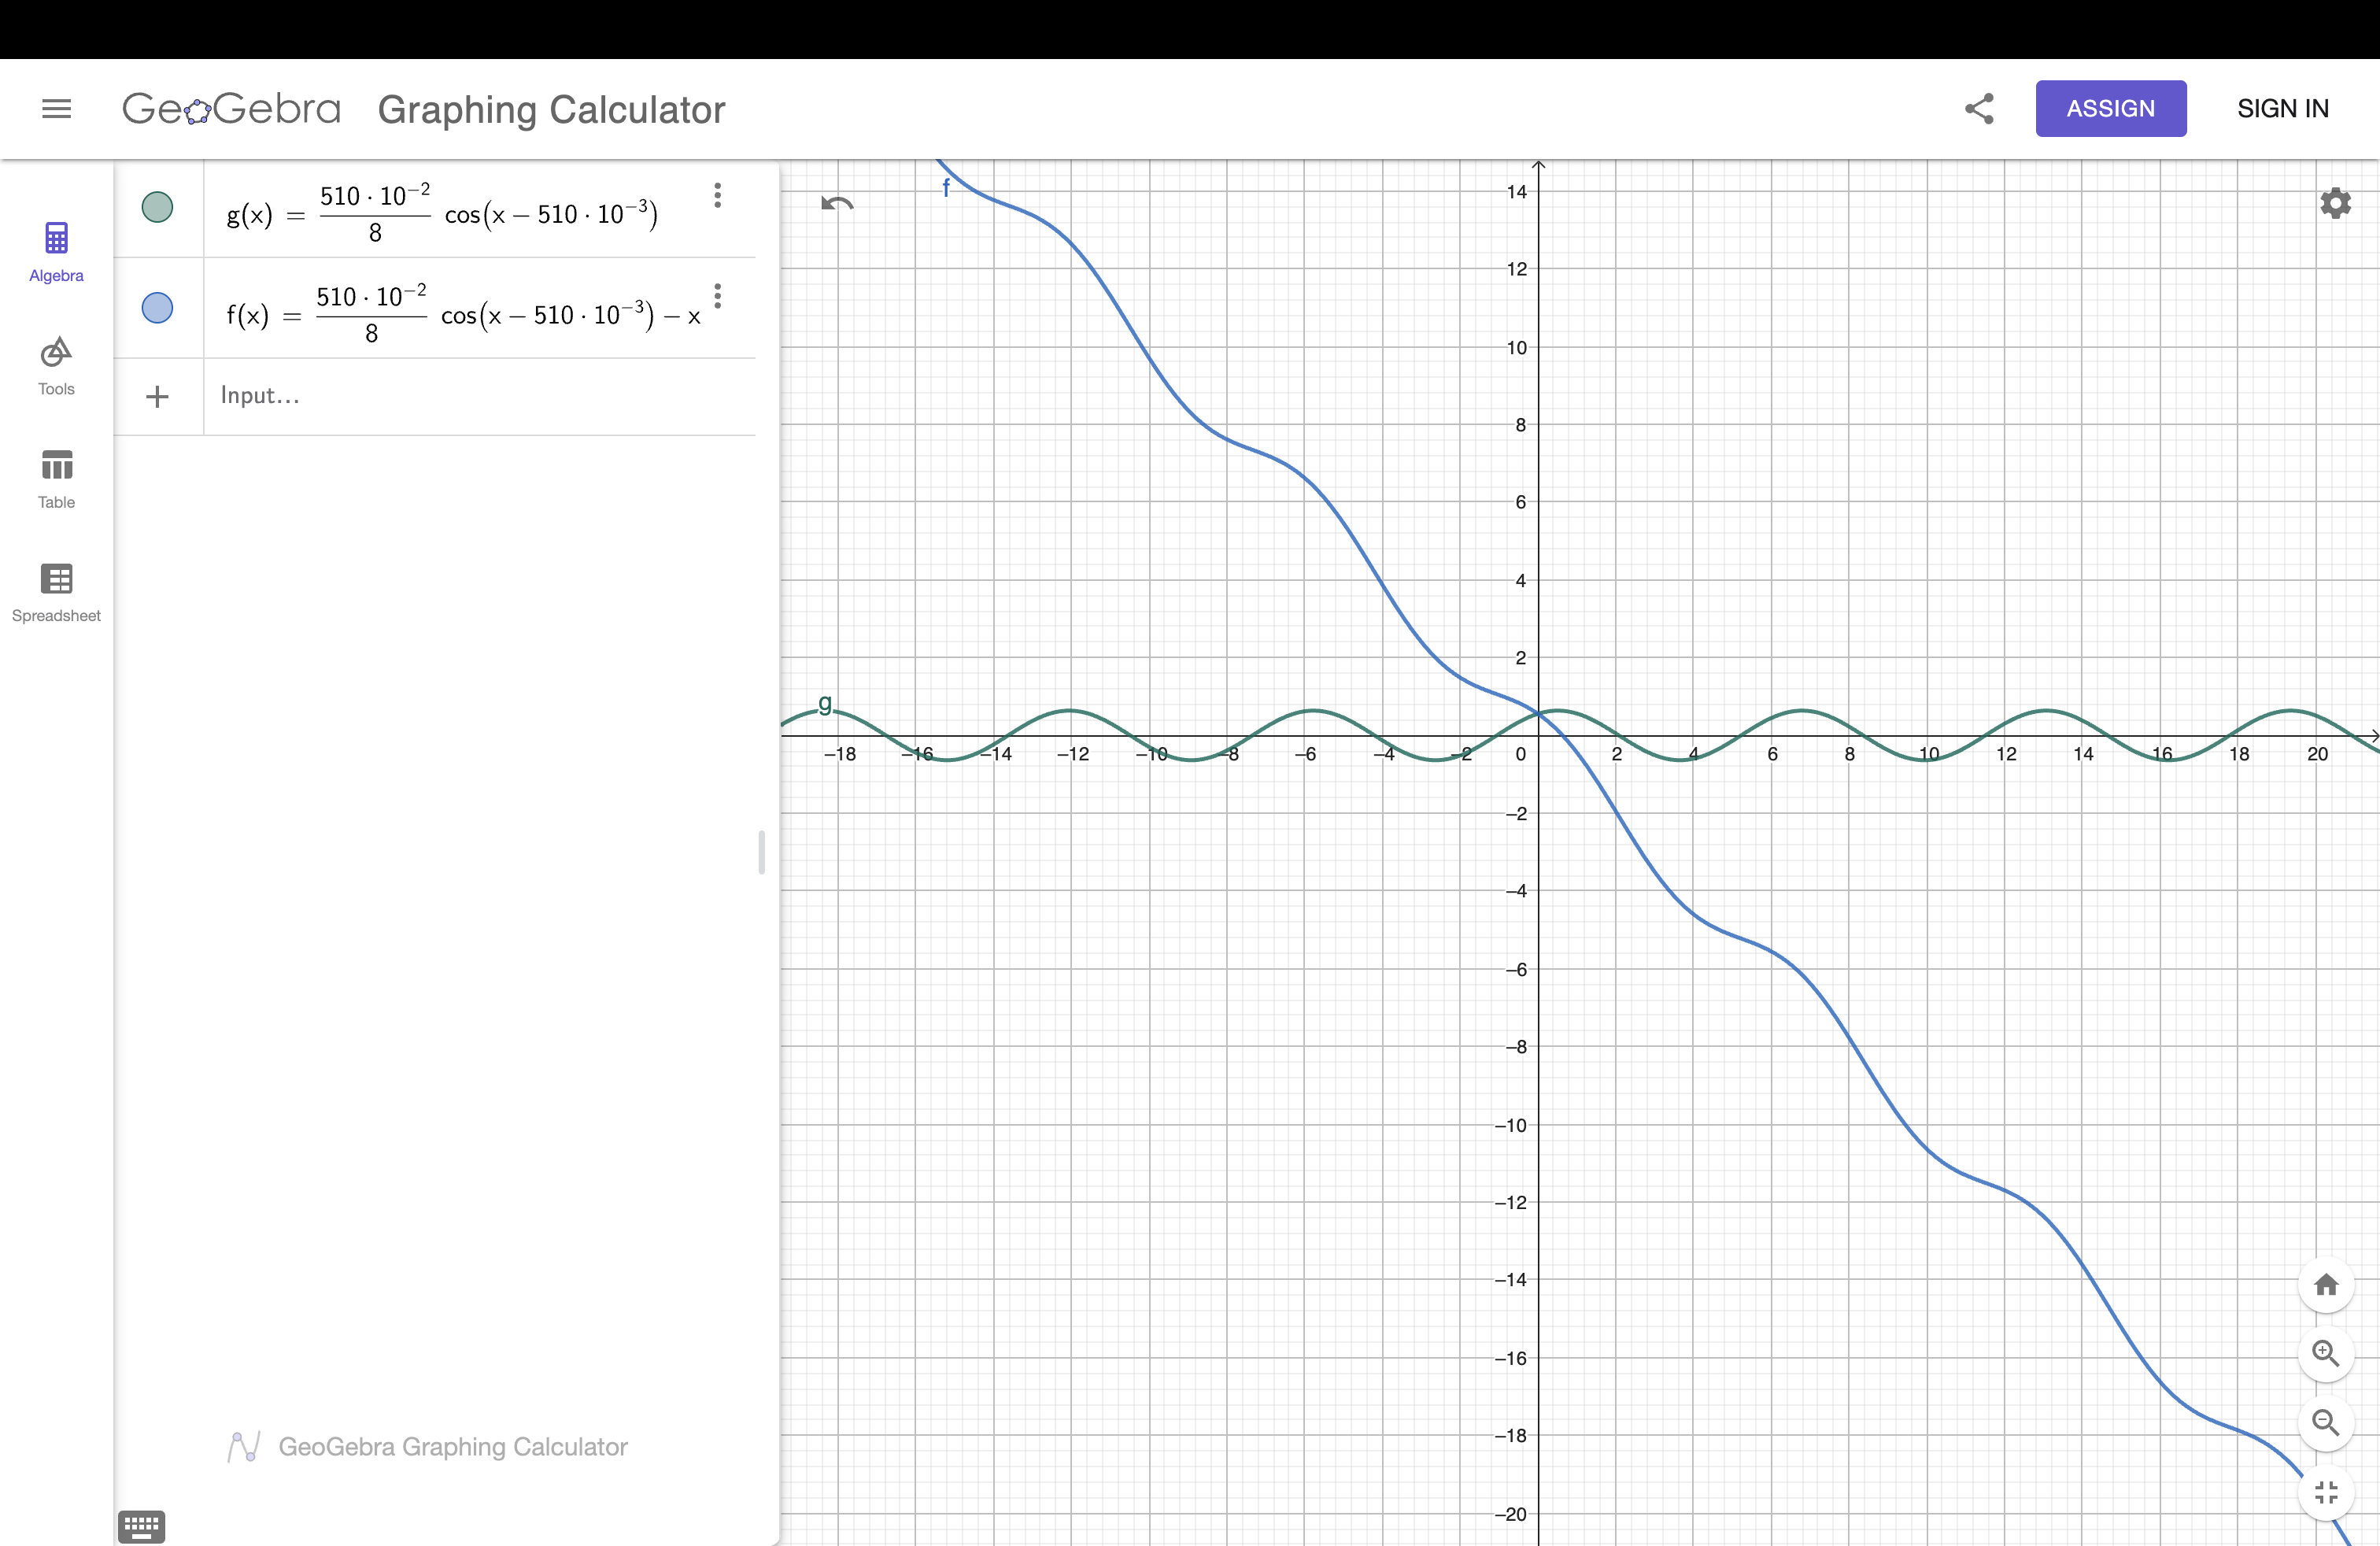
\includegraphics[width=\textwidth]{Figures/0. General/2.1.1.png}
        \caption{Gráfico de $f(x)$ y $g(x)$}
        \label{fig: Grafico de f(x) y g(x)}
    \end{subfigure}
\end{figure}

\subsection{Gráfico de $f(x)$ y $g(x)$ con intervalo $[0,2]$}
\begin{figure}[H]
    \centering
    \begin{subfigure}[b]{\textwidth}
        \centering
        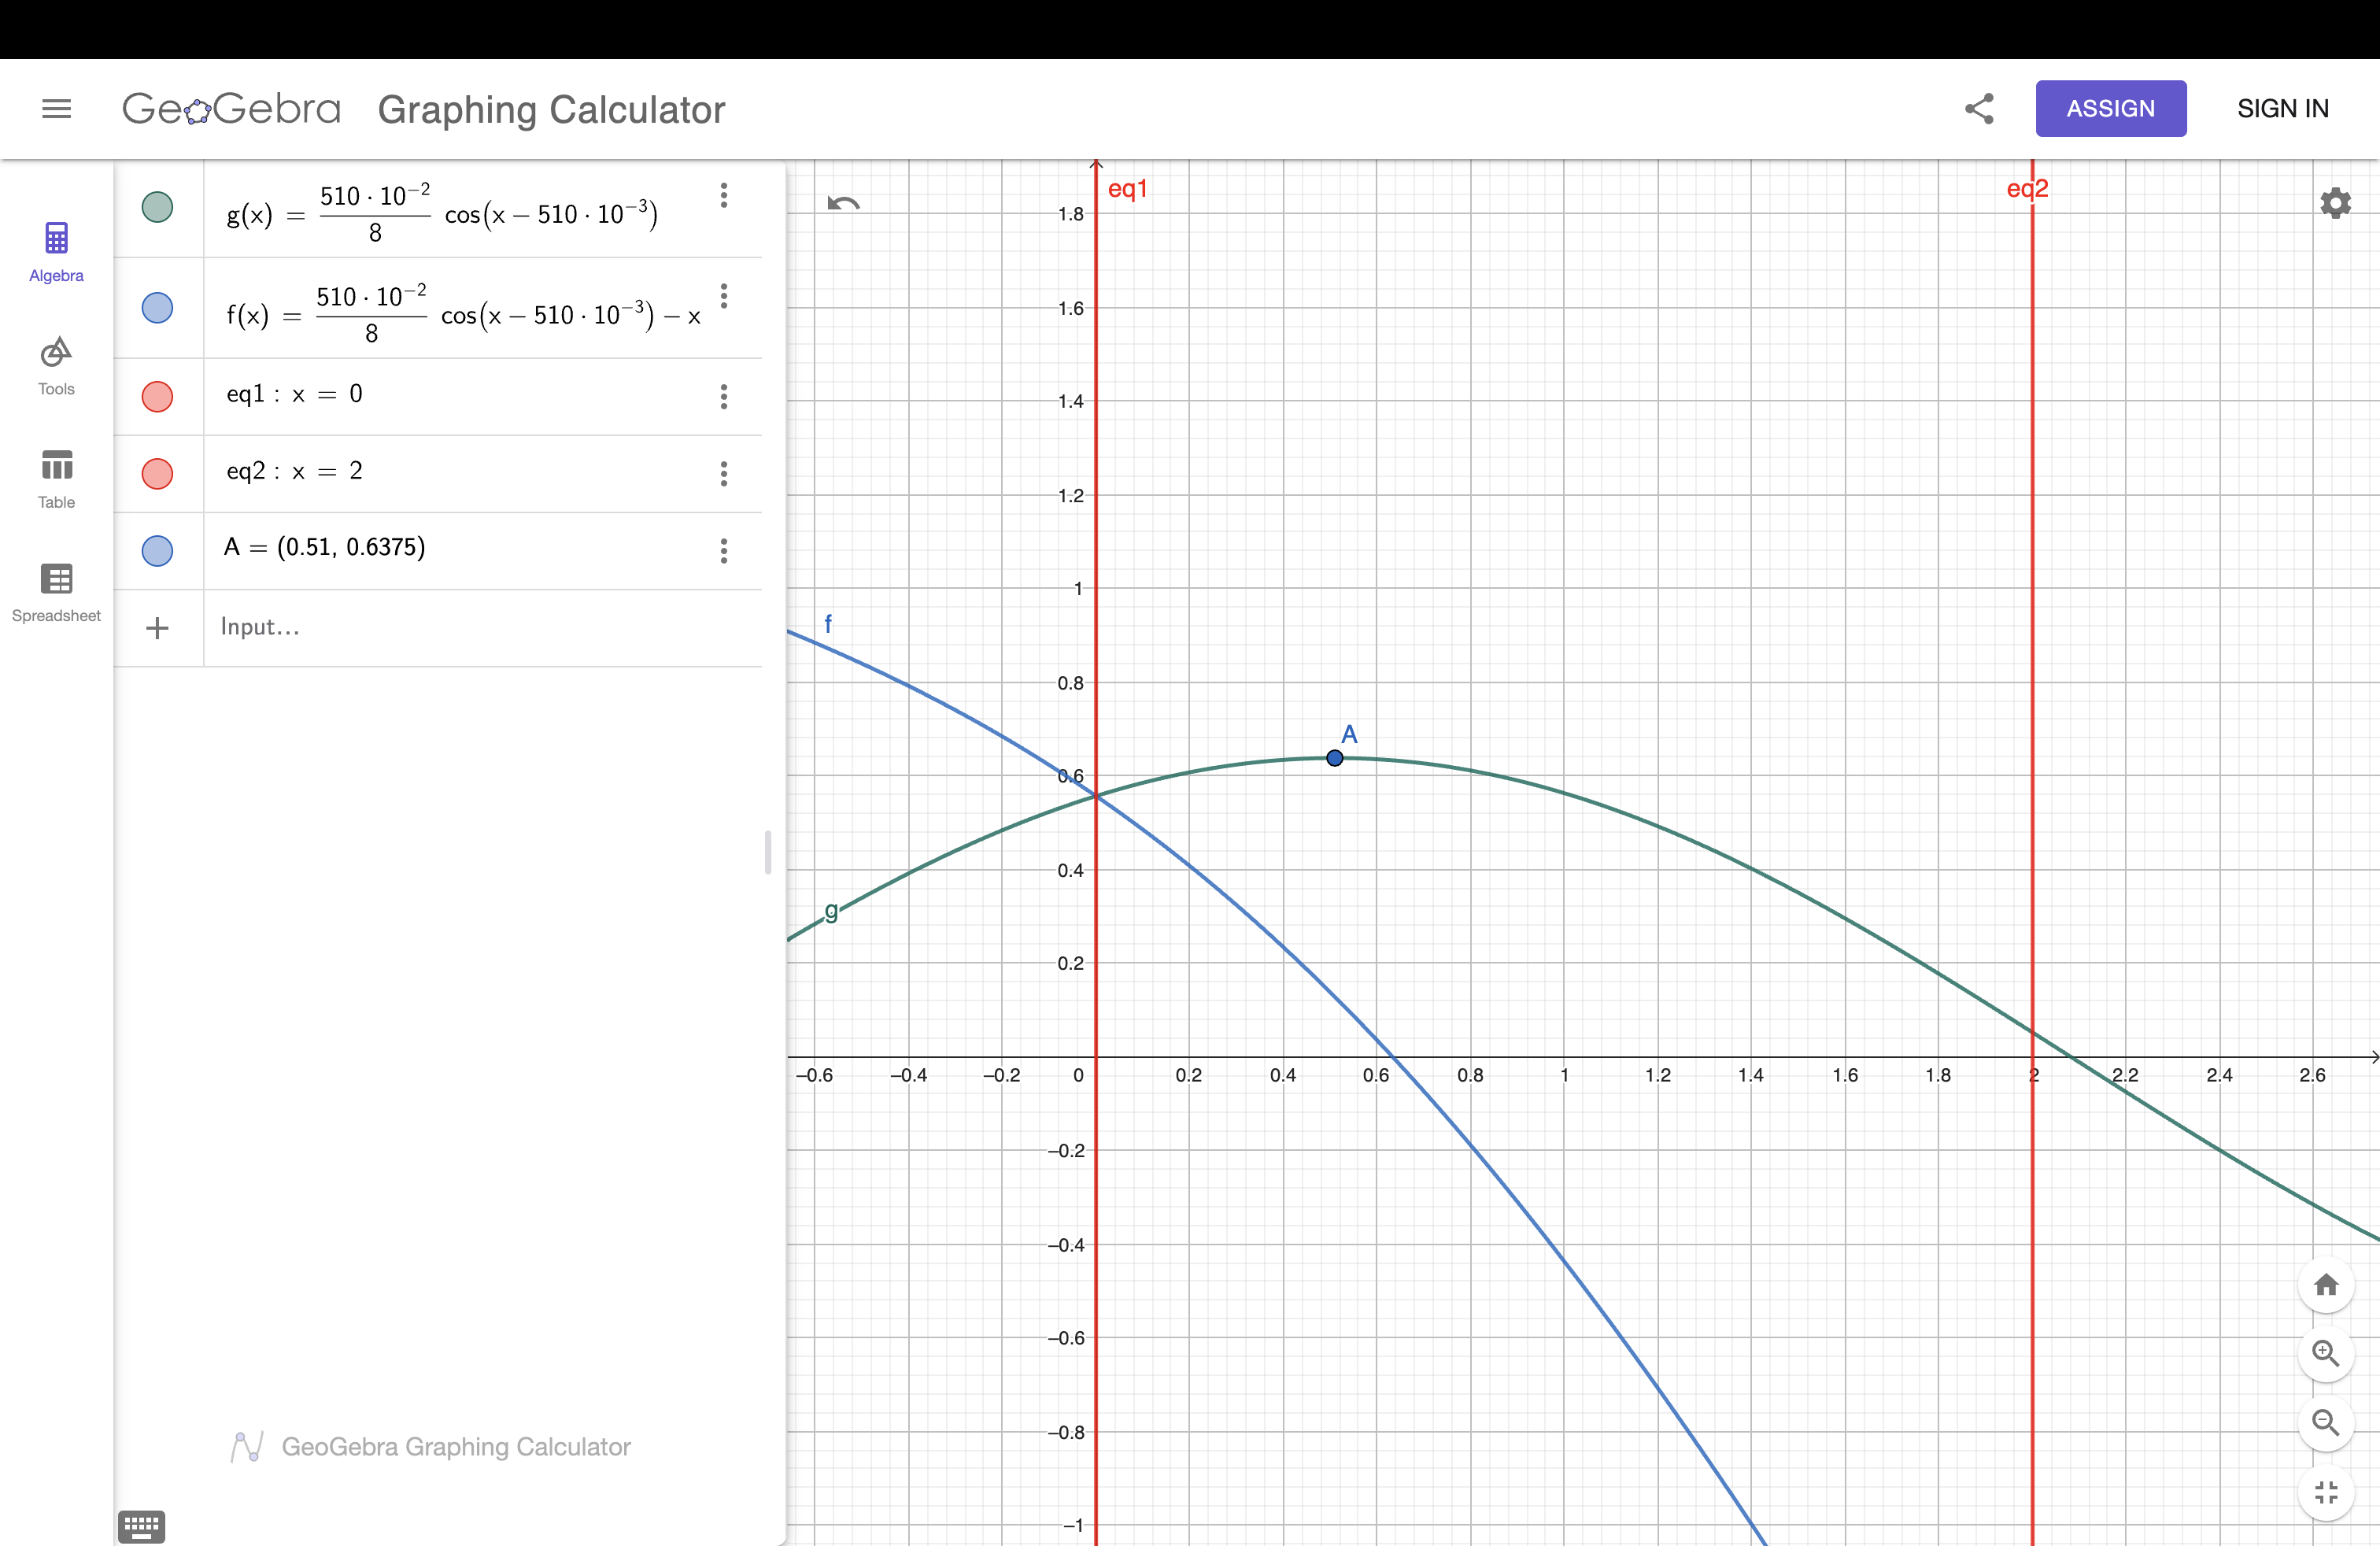
\includegraphics[width=\textwidth]{Figures/0. General/2.1.2.png}
        \caption{Gráfico de $f(x)$ y $g(x)$ con intervalo $[0,2]$}
        \label{fig: Grafico de f(x) y g(x) con intervalo [0,2]}
    \end{subfigure}
\end{figure}

\subsection{Análisis Gráfico en el intervalo \([0,2]\)}

Para que el método de punto fijo converja en un intervalo dado, se acostumbra verificar tres condiciones:

\begin{enumerate}
  \item \textbf{Continuidad de \(g(x)\) en \([0,2]\).}
  En la Figura \ref{fig: Grafico de f(x) y g(x)} y \ref{fig: Grafico de f(x) y g(x) con intervalo [0,2]}, puede apreciarse que \(g(x)\) (curva verde) es continua en el rango mostrado, pues está definida para todos los \(x\) entre 0 y 2.

  \item \textbf{Auto-mapeo:} \(g(x)\) debe enviar valores de \([0,2]\) de vuelta a \([0,2]\).
  Gráficamente, esto se observa si, para todo \(x\in[0,2]\), la imagen \(g(x)\) (altura en el eje \(y\)) se encuentra también entre 0 y 2. Se puede verificar que:
  \[
    0 \;\le\; g(x) \;=\;0.6375 \,\cos(x-0.510) \;\le\;2
    \quad\text{para }x\in[0,2],
  \]
  al menos de forma aproximada revisando que el máximo de \(0.6375 \cos(\dots)\) en ese rango no supere 2 y no se haga negativa de manera drástica. En la gráfica, se ve que \(g(x)\) permanece por encima de 0 y por debajo de 1 alrededor de ese intervalo.

  \item \textbf{Condición de contracción:} \(\max_{x\in [0,2]} \lvert g'(x)\rvert < 1.\)
  Para \(g(x) = 0.6375\,\cos(x - 0.510)\), la derivada es
  \[
    g'(x) \;=\; -\,0.6375\,\sin\bigl(x - 0.510\bigr).
  \]
  El valor absoluto es \(\lvert g'(x)\rvert = 0.6375\,\lvert\sin(\dots)\rvert \le 0.6375 < 1\) para todo \(x\). Por ende, en \([0,2]\), se cumple \(\lvert g'(x)\rvert<1\).

\end{enumerate}

\noindent
\textbf{Conclusión gráfica:}  
Dado que las tres condiciones se satisfacen en \([0,2]\), existe un único punto de intersección entre la gráfica de \(y=g(x)\) y la recta \(y=x\). Dicho punto es precisamente la solución de \(x = g(x)\), lo que confirma la convergencia al valor hallado (\(x\approx 0.6327\)) y explica por qué el método de punto fijo funcionó correctamente en ese intervalo.

\section{Kingping (1 pt)}

El Alcalde Kingping también se encuentra enfermo de la cabeza y decide robarse
la estrategia de Daredevil para saber que tan enfermo está, pero usa la misma
función $f(x)$ el valor de $A=999$, y a pesar de que el método le converge,
siempre le dan más iteraciones que a Daredevil.
Explique a Kingpin a que se debe esto, desde su conocimiento del método, antes
de que los termine asesinando a Daredevil y a usted.


\subsection{Gráfico de $f(x)$ y $g(x)$}
\begin{figure}[H]
    \centering
    \begin{subfigure}[b]{\textwidth}
        \centering
        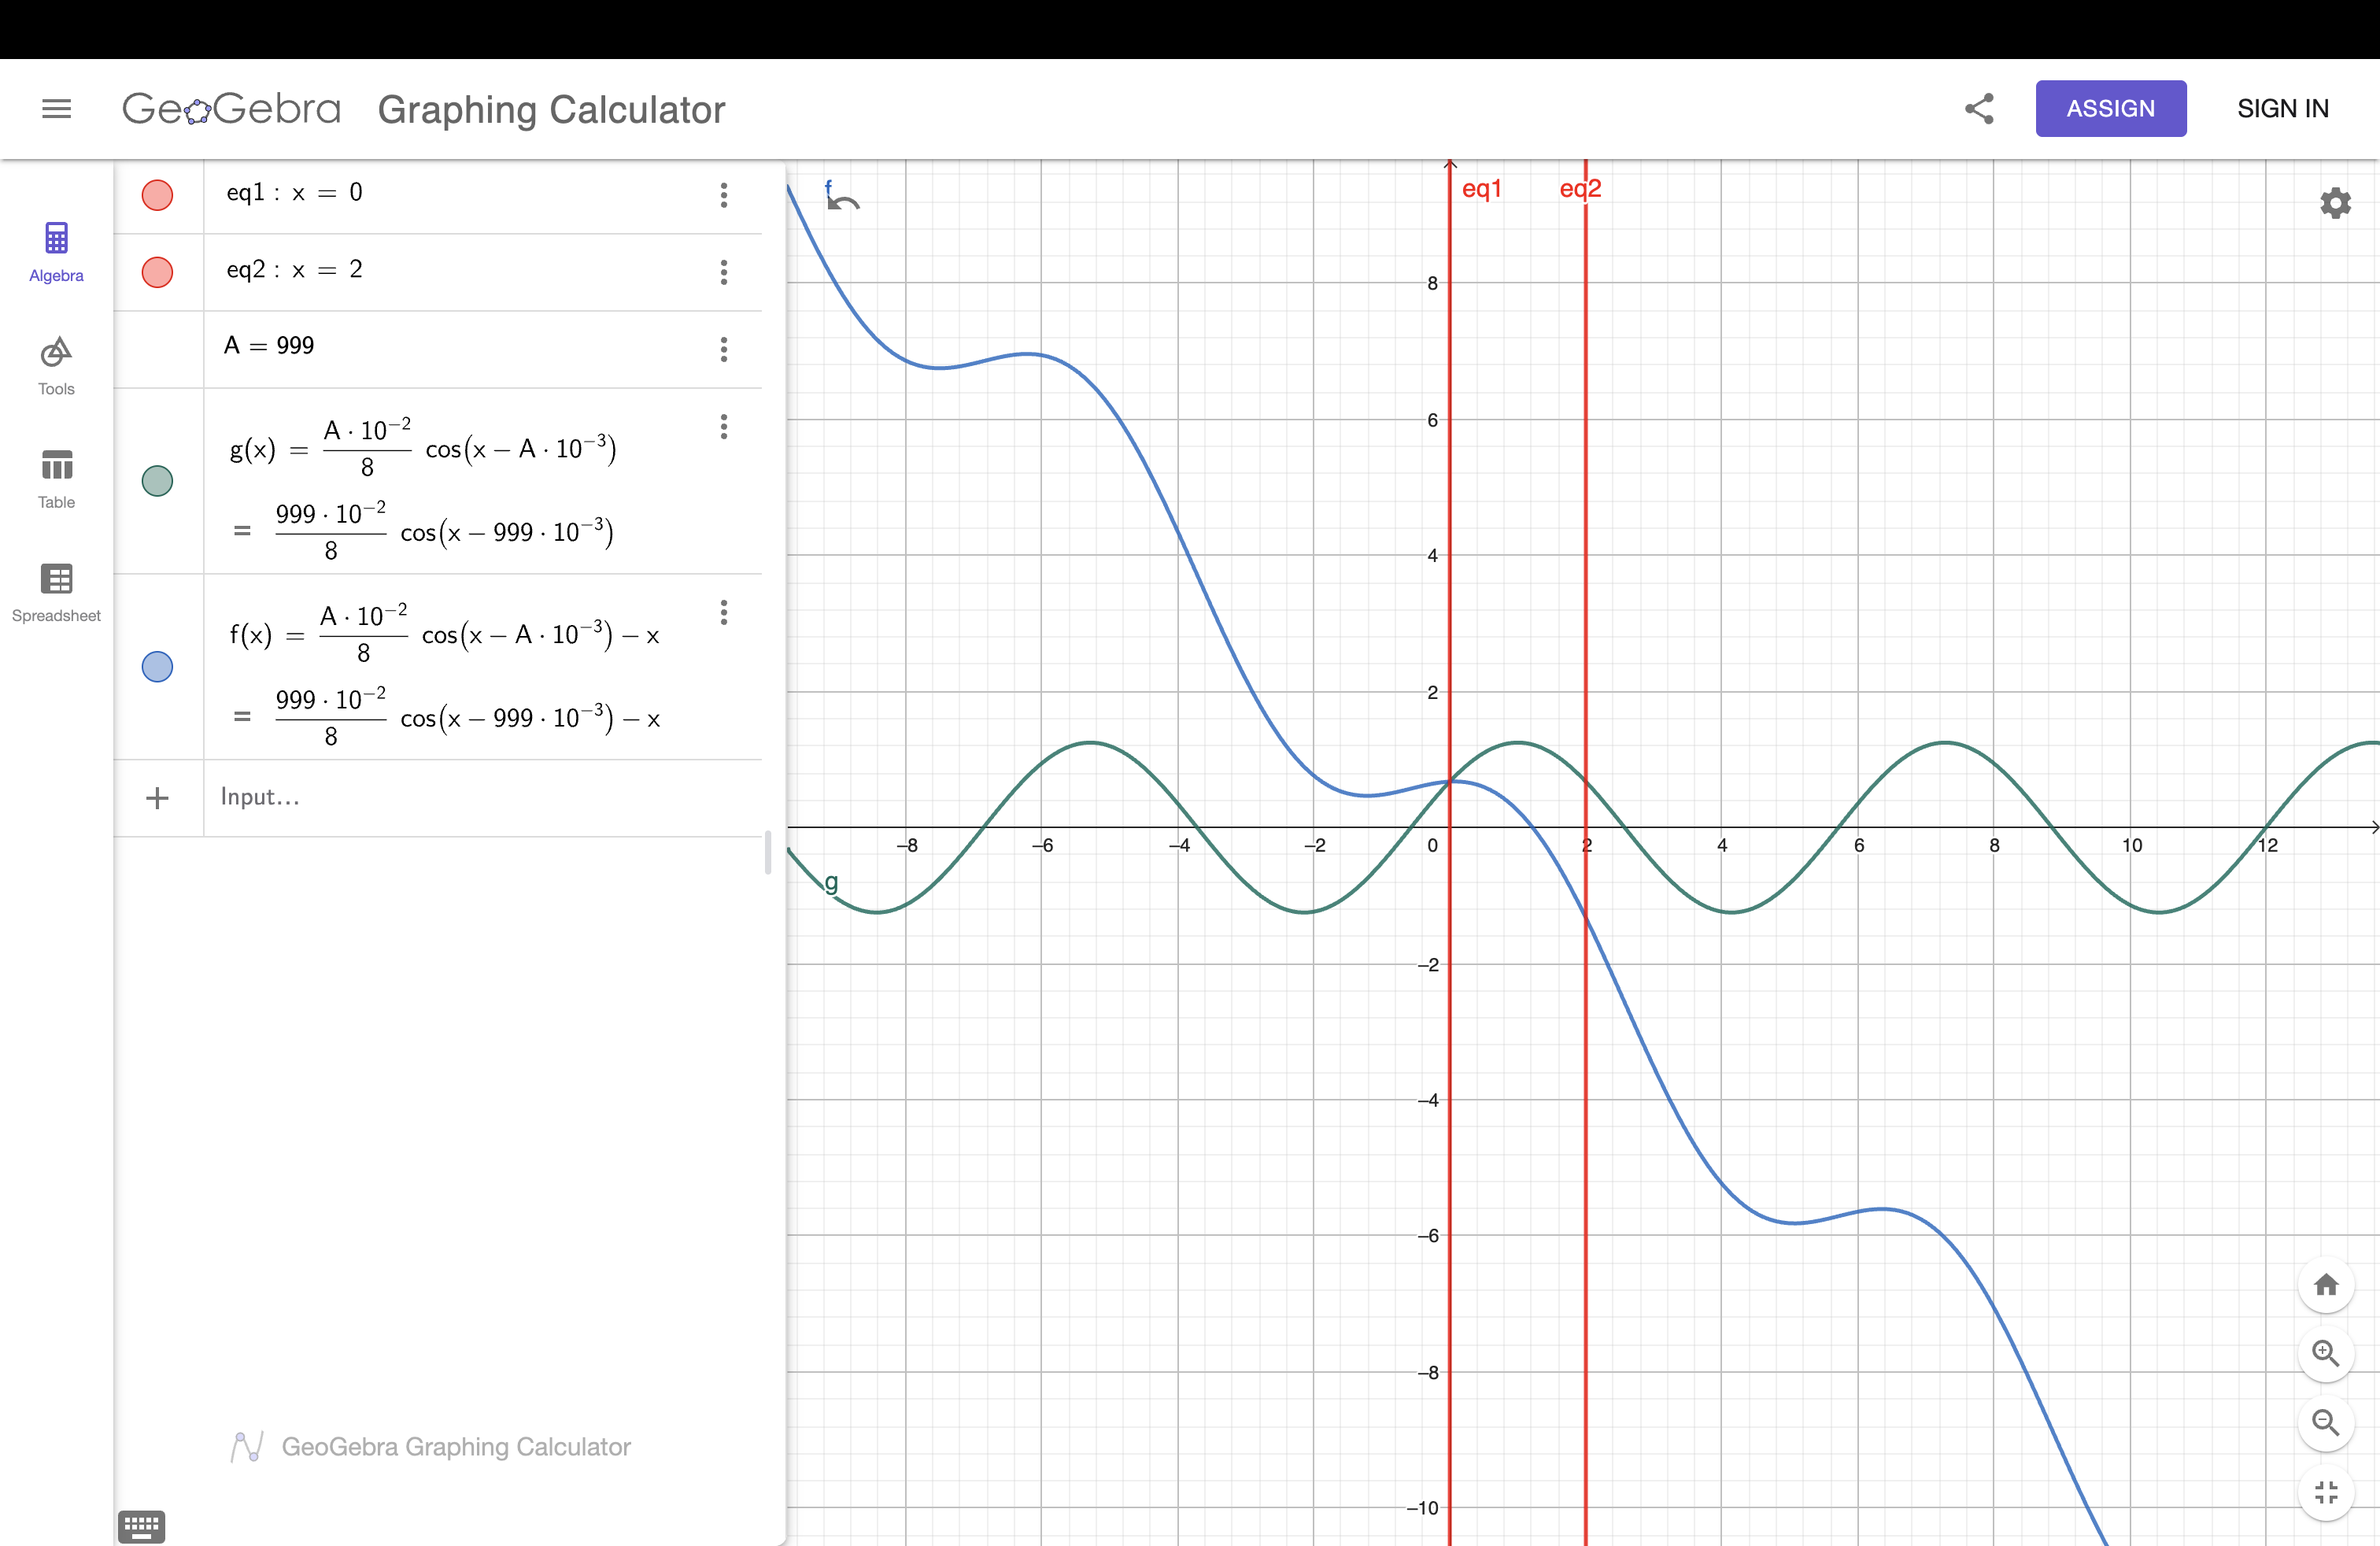
\includegraphics[width=\textwidth]{Figures/0. General/3.1.1.png}
        \caption{Gráfico de $f(x)$ y $g(x)$}
        \label{fig: Grafico de f(x) y g(x) de Kingping}
    \end{subfigure}
\end{figure}

\subsection{Gráfico de $f(x)$ y $g(x)$ con intervalo $[0,2]$}
\begin{figure}[H]
    \centering
    \begin{subfigure}[b]{\textwidth}
        \centering
        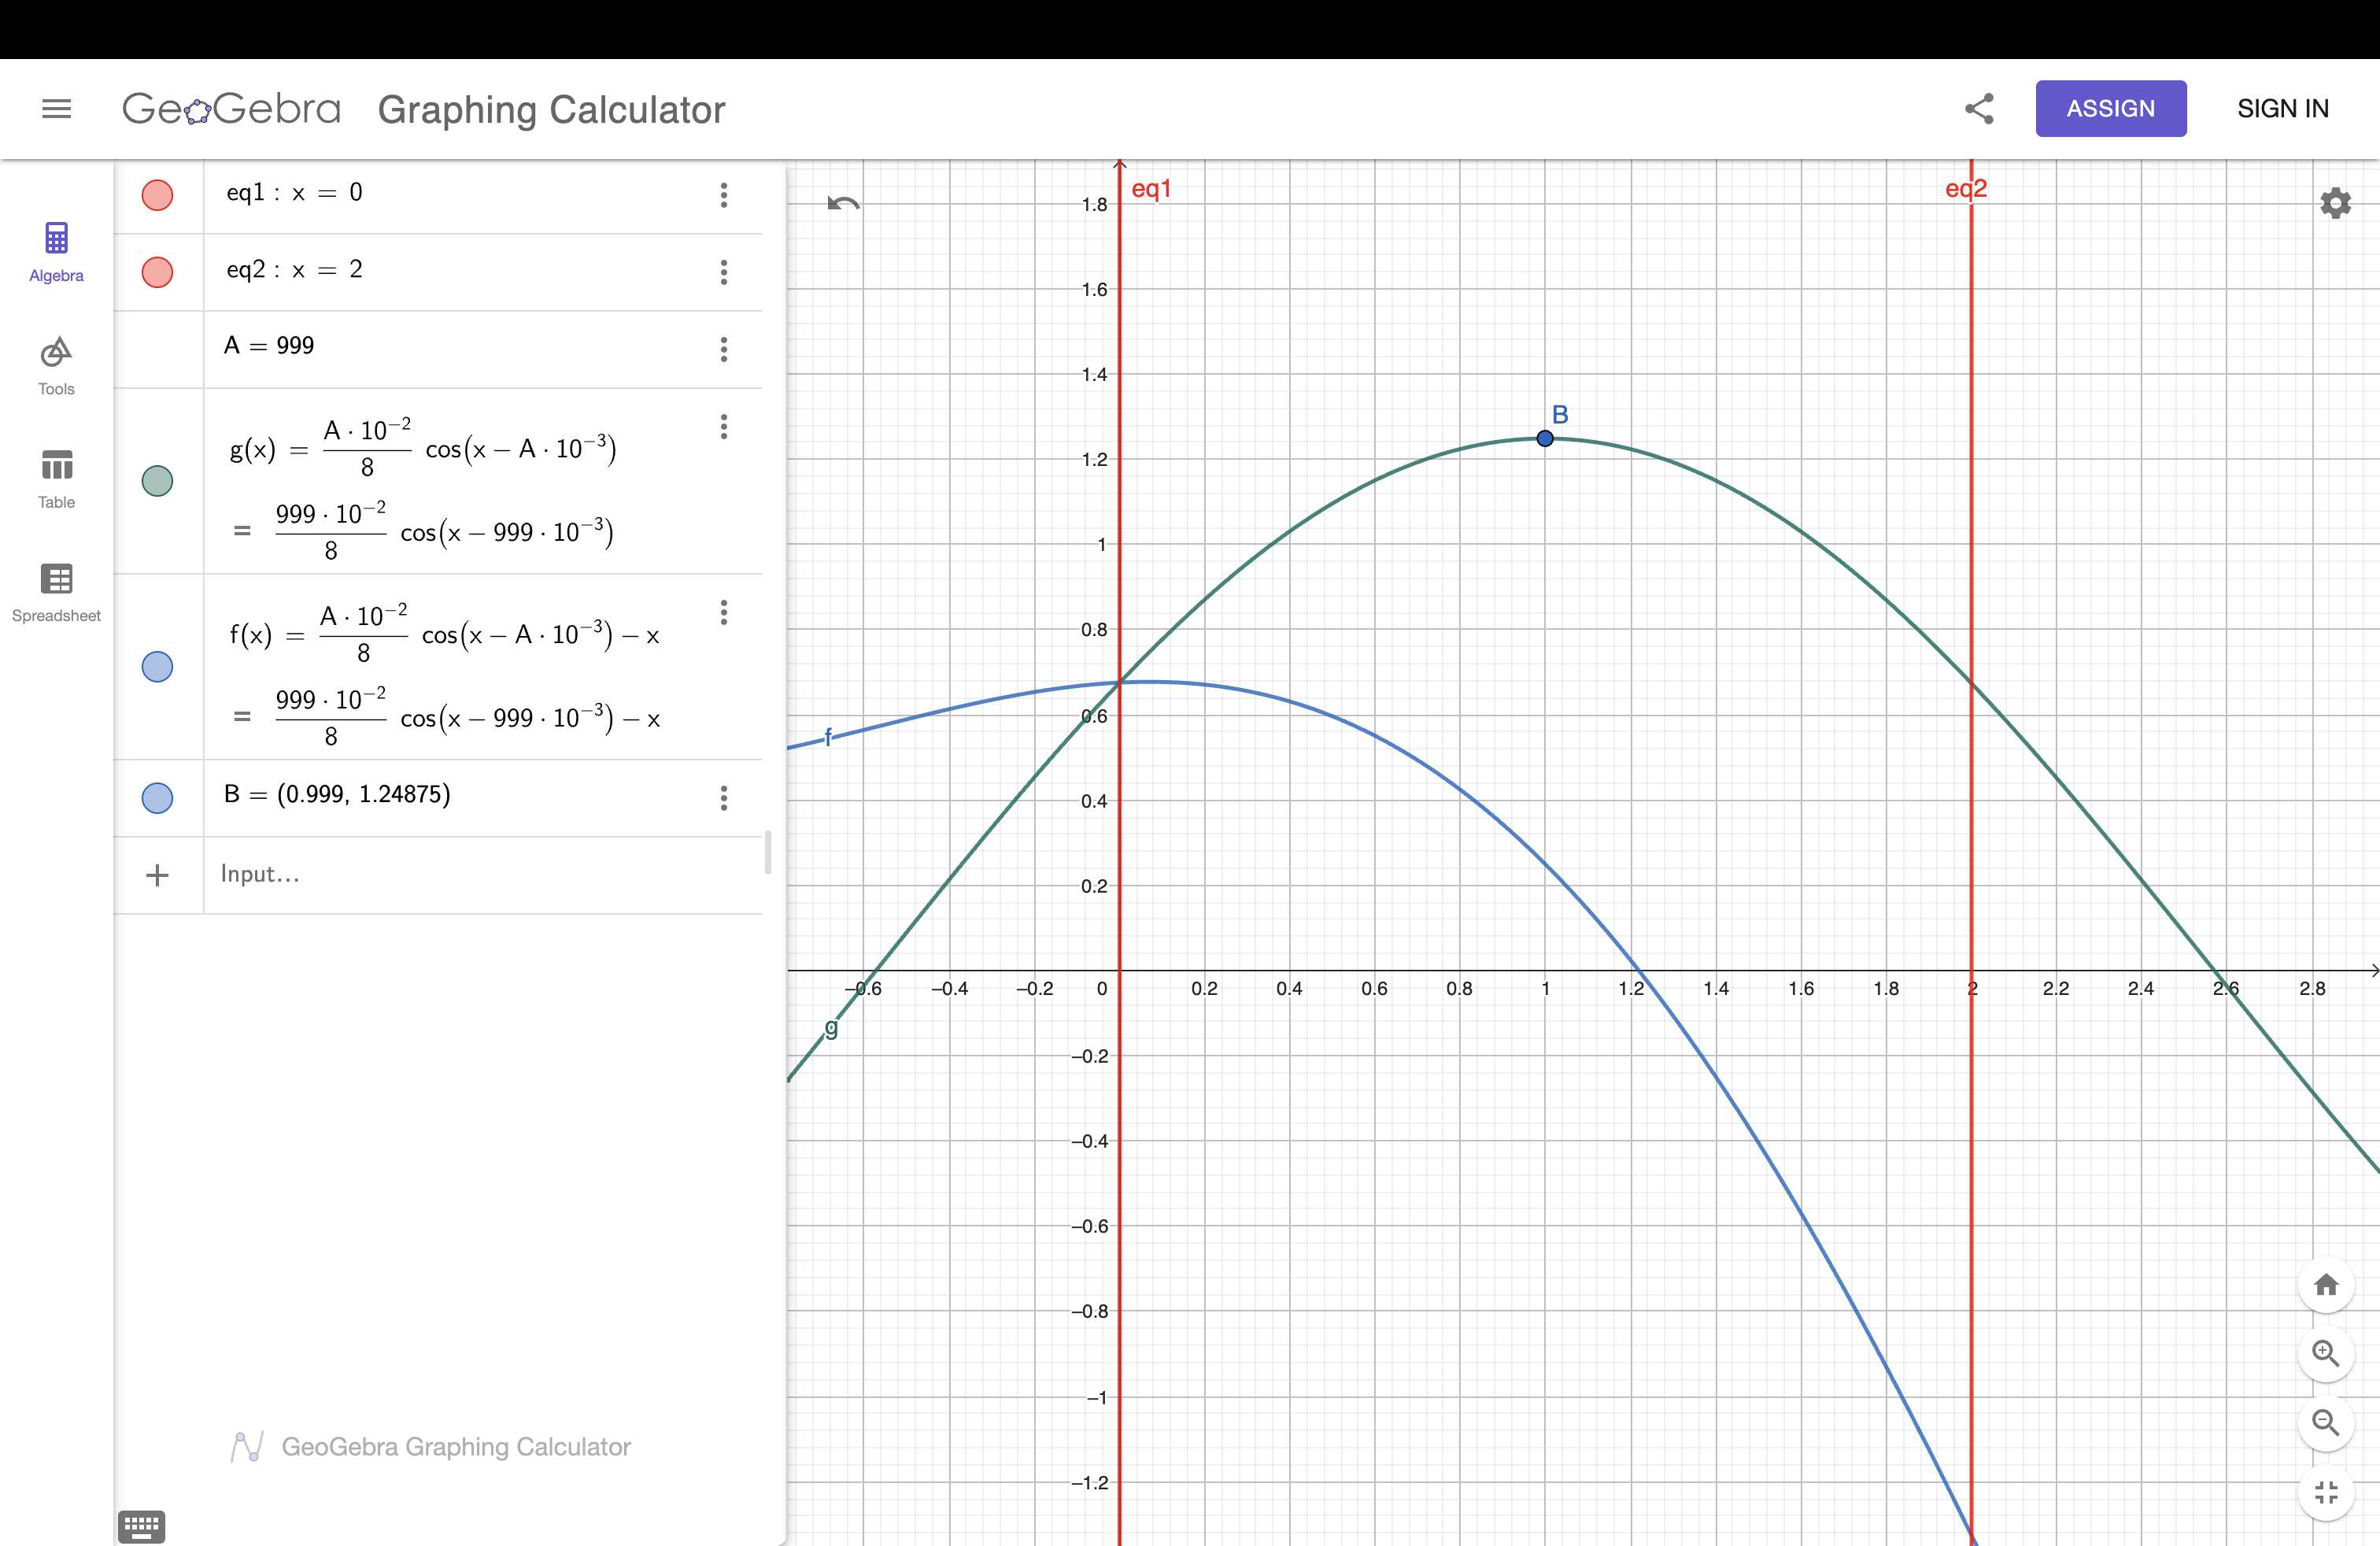
\includegraphics[width=\textwidth]{Figures/0. General/3.1.2.png}
        \caption{Gráfico de $f(x)$ y $g(x)$ con intervalo $[0,2]$}
        \label{fig: Grafico de f(x) y g(x) con intervalo [0,2] de Kingping}
    \end{subfigure}
\end{figure}

\subsection{Explicación para Kingpin}

En el caso de Kingpin, se vuelve a usar la ecuación 
\[
f(x) \;=\; \frac{A \times 10^{-2}}{8}\,\cos\bigl(x - A \times 10^{-3}\bigr) \;-\; x
\]
pero con \(A=999\). Entonces la función de iteración toma la forma
\[
g(x) \;=\;\frac{999 \times 10^{-2}}{8}\,\cos\bigl(x - 999\times 10^{-3}\bigr)
\;=\;\frac{9.99}{8}\,\cos(x - 0.999).
\]
Nótese que \(\frac{9.99}{8}\approx 1.24875\). Por tanto, su derivada
\[
g'(x) \;=\;-\,\frac{9.99}{8}\,\sin\bigl(x - 0.999\bigr)
\]
tiene un valor absoluto máximo cercano a \(1.24875\). Mientras más cerca está \(\lvert g'(x)\rvert\) de \(1\), más lenta tiende a ser la convergencia del método de punto fijo (incluso puede divergir si supera \(1\) en todo el intervalo). 

En este problema, aunque sigue habiendo un rango donde \(\lvert g'(x)\rvert<1\) y el método converge, la constante de contracción es \textit{menor} que la del caso de Daredevil (para \(A=510\)), lo que significa que cada iteración reduce el error más lentamente. Por eso Kingpin observa que, aunque también llega a una solución, \textbf{necesita más iteraciones} que Daredevil para alcanzar la misma tolerancia.



\section{Traje de Daredevil (1 pt)}

Al final, Daredevil descubre que una farmacéutica está escondiendo los
medicamentos para la ceguera, por lo que decide si armar el mierdero, sin
embargo no sabe qué traje ponerse. Si la probabilidad de ponerse el traje negro es 
\(x_1\), el rojo es \(x_2\) y el amarillo es \(x_3\), indique claramente qué
probabilidad tiene en cada traje, resolviendo el siguiente sistema de ecuaciones
con el método de pivoteo total, y calcule el error escalar en norma infinito. 
Se da que \(\alpha = 0\):

\begin{align*}
   \alpha x_1 + 10x_2 + 30x_3 &= 70,\\
    -8x_1 + 6x_2 - \alpha x_3 &= 80,\\
    9x_1 + x_2 - 12x_3 &= 90.
\end{align*}

Con \(\alpha = 0\), el sistema queda:

\begin{align*}
  0\cdot x_1 + 10x_2 + 30x_3 &= 70,\\
   -8x_1 + 6x_2 + 0\cdot x_3 &= 80,\\
   9x_1 + x_2 - 12x_3 &= 90.
\end{align*}

\subsection{Solución del sistema por Pivoteo Total (con \(\alpha = 0\))}

Dado el sistema:
\[
\begin{cases}
0\,x_1 + 10\,x_2 + 30\,x_3 = 70,\\
-8\,x_1 + 6\,x_2 + 0\,x_3 = 80,\\
9\,x_1 + 1\,x_2 - 12\,x_3 = 90,
\end{cases}
\]
deseamos encontrar \((x_1,x_2,x_3)\) usando \textbf{pivoteo total}, y luego calcular el \textbf{error escalar en norma infinito}.

\subsubsection{Formar la matriz aumentada}

\[
A =
\begin{pmatrix}
0 & 10 & 30\\
-8 & 6 & 0\\
9 & 1 & -12
\end{pmatrix},
\quad
\mathbf{b}=
\begin{pmatrix}
70\\
80\\
90
\end{pmatrix},
\quad
[A|\mathbf{b}]=
\begin{pmatrix}
0 & 10 & 30 & 70\\
-8 & 6 & 0 & 80\\
9 & 1 & -12 & 90
\end{pmatrix}.
\]

Definimos el \emph{vector índice de columnas} \(\texttt{mark} = (1,2,3)\) para llevar seguimiento de los intercambios de columnas.

\subsubsection{Primera búsqueda de pivote (etapa \(k=1\))}

Buscamos el elemento de valor absoluto máximo en la submatriz de filas 1--3 y columnas 1--3.  
Las magnitudes son:
\[
|0|=0,\;\;|10|=10,\;\;|30|=30,\quad
|{-8}|=8,\;\;|6|=6,\;\;|0|=0,\quad
|9|=9,\;\;|1|=1,\;\;|{-12}|=12.
\]
El mayor es \(30\), en la fila 1, columna 3.

\begin{itemize}
\item \textbf{Intercambio de filas}: 
   la fila pivote es 1, y la del mayor es también 1, así que no se intercambian filas.

\item \textbf{Intercambio de columnas}:
   la columna pivote es 1, pero el valor mayor está en la col.3.
   Intercambiamos col.1 \(\leftrightarrow\) col.3 en toda la matriz, y también en \(\texttt{mark}\).

   \[
   \texttt{mark}=(1,2,3)\;\;\longrightarrow\;\;\texttt{mark}=(3,2,1).
   \]

   Tras el intercambio, la matriz aumentada pasa a:
   \[
   [A|\mathbf{b}]
   \;\longrightarrow\;
   \begin{pmatrix}
   30 & 10 & 0 & 70\\
   0 & 6 & -8 & 80\\
   -12 & 1 & 9 & 90
   \end{pmatrix}.
   \]
\end{itemize}

Ahora el pivote es \(a_{11}=30\).

\textbf{Eliminación debajo del pivote}:
\[
\text{F2} \leftarrow \text{F2} - \frac{0}{30}\,\text{F1} \quad(\text{sin cambio}),
\]
\[
\text{F3} \leftarrow \text{F3} - \frac{-12}{30}\,\text{F1} 
= \text{F3} + 0.4\,\text{F1}.
\]
En la práctica,
\[
\text{F3}=(\,{-12},\,1,\,9,\,90),\quad
0.4\,\text{F1}=(\,12,\,4,\,0,\,28).
\]
Sumando:
\[
\text{F3}\leftarrow(0,\,5,\,9,\,118).
\]
Se obtiene:
\[
[A|\mathbf{b}]\;\to\;
\begin{pmatrix}
30 & 10 & 0 & 70\\
0 & 6 & -8 & 80\\
0 & 5 & 9 & 118
\end{pmatrix}.
\]

\subsubsection{Segunda búsqueda de pivote (etapa \(k=2\))}

Tomamos la submatriz de filas 2--3 y columnas 2--3. Sus valores:
\[
|6|=6, \;|{-8}|=8,
\quad
|5|=5,\;|9|=9.
\]
El mayor es \(8\) (es \(\lvert -8\rvert\)) en la fila 2, col.3.

\begin{itemize}
\item \textbf{Intercambio de filas}:
   la fila pivote es 2 y la del mayor también 2, así que no se intercambian filas.
\item \textbf{Intercambio de columnas}:
   la columna pivote es 2, y la del mayor es 3. Intercambiamos col.2 \(\leftrightarrow\) col.3, y se actualiza \(\texttt{mark}\):
   \[
   \texttt{mark}=(3,2,1)\;\;\longrightarrow\;\;\texttt{mark}=(3,1,2).
   \]
   La matriz aumenta pasa a:
   \[
   \begin{pmatrix}
   30 & 0 & 10 & 70\\
   0 & -8 & 6 & 80\\
   0 & 9 & 5 & 118
   \end{pmatrix}.
   \]
\end{itemize}

El pivote es \(-8\). Eliminamos en la fila 3:
\[
\text{F3} \leftarrow \text{F3} - \frac{9}{-8}\,\text{F2}
= \text{F3} + \frac{9}{8}\,\text{F2}.
\]
\(\text{F2}=(\,0,\,-8,\,6,\,80)\). Entonces
\[
\frac{9}{8}\,\text{F2}=(0,\,-9,\,6.75,\,90),
\]
y al sumar con \(\text{F3}=(0,\,9,\,5,\,118)\) obtenemos
\[
\text{F3}\leftarrow(0,\,0,\,11.75,\,208).
\]
La matriz queda:
\[
[A|\mathbf{b}]\;\to\;
\begin{pmatrix}
30 & 0 & 10 & 70\\
0 & -8 & 6 & 80\\
0 & 0 & 11.75 & 208
\end{pmatrix}.
\]

\subsubsection{Tercera búsqueda (etapa \(k=3\))}

La submatriz final es el único elemento \(11.75\). No se requiere intercambio.
Se tiene la forma triangular superior terminada.

\subsubsection{Resolución por sustitución regresiva}

\begin{enumerate}
\item 3\textsuperscript{a} fila:
\[
11.75\,x_{\text{col3}}=208 \quad\Longrightarrow\quad
x_{\text{col3}}=\frac{208}{11.75}\approx 17.70.
\]
\item 2\textsuperscript{a} fila:
\[
-8\,x_{\text{col2}} + 6\,x_{\text{col3}}=80 \quad\Longrightarrow\quad
-8\,x_{\text{col2}} + 6(17.70)=80.
\]
\[
-8\,x_{\text{col2}} +106.2=80
\;\Longrightarrow\;
-8\,x_{\text{col2}}=-26.2
\;\Longrightarrow\;
x_{\text{col2}}=3.275.
\]
\item 1\textsuperscript{a} fila:
\[
30\,x_{\text{col1}} +10\,x_{\text{col3}}=70
\quad\Longrightarrow\quad
30\,x_{\text{col1}} +10(17.70)=70.
\]
\[
30\,x_{\text{col1}} +177=70
\;\Longrightarrow\;
30\,x_{\text{col1}}=-107
\;\Longrightarrow\;
x_{\text{col1}}=-\frac{107}{30}\approx -3.5667.
\]
\end{enumerate}

\[
x_{\text{col1}}\approx-3.5667,\quad
x_{\text{col2}}\approx3.275,\quad
x_{\text{col3}}\approx17.70.
\]

\subsubsection{Reinterpretar variables según \(\texttt{mark}\)}

Al final, \(\texttt{mark}=(3,1,2)\). Esto significa:
\[
\begin{aligned}
&\texttt{mark}(1)=3 \;\;\Rightarrow\; 
x_{\text{col1}}\;\text{es en realidad}\; x_3,\\
&\texttt{mark}(2)=1 \;\;\Rightarrow\; 
x_{\text{col2}}\;\text{es en realidad}\; x_1,\\
&\texttt{mark}(3)=2 \;\;\Rightarrow\; 
x_{\text{col3}}\;\text{es en realidad}\; x_2.
\end{aligned}
\]

Por tanto, en orden \((x_1,x_2,x_3)\):
\[
x_1 = 3.275,\quad
x_2 = 17.70,\quad
x_3 = -3.5667.
\]

\subsubsection{Probabilidades en cada traje}

Con \(x_1\) (negro), \(x_2\) (rojo), \(x_3\) (amarillo), resulta:
\[
\boxed{
x_1\approx 3.275,\quad
x_2\approx 17.70,\quad
x_3\approx -3.5667.
}
\]
Si se pretendiera que las \(x_i\) fuesen probabilidades \((0\le x_i\le1)\), veríamos que la solución no se ajusta a ese sentido estricto; el problema da valores reales sin forzar la suma a 1 ni la positividad.

\subsubsection{Cálculo del error escalar en norma infinito}

Usualmente, si no contamos con una solución exacta distinta, medimos el \emph{residuo}:
\[
\mathbf{r}=A\,\tilde{\mathbf{x}}-\mathbf{b},
\quad
\|\mathbf{r}\|_\infty=\max\{|r_1|,|r_2|,|r_3|\}.
\]
Substituyendo \(\tilde{x}_1=3.275\), \(\tilde{x}_2=17.70\), \(\tilde{x}_3=-3.5667\), en las ecuaciones:
\[
\begin{aligned}
0\cdot x_1 +10\,x_2 +30\,x_3 &=\,10(17.70)+30(-3.5667)=177-107=70,\\
-8\,x_1 +6\,x_2 +0 &=\,-8(3.275)+6(17.70)= -26.2 +106.2=80,\\
9\,x_1 + x_2 -12\,x_3 &=\,9(3.275) + 17.70 -12(-3.5667)=29.475+17.70+42.8=89.975\approx90.
\end{aligned}
\]
Las ligeras diferencias se deben a redondeo, resultando en un error del orden \(10^{-5}\) o menor. Por ende,
\[
\boxed{\|\mathbf{r}\|_\infty \approx 0\;\;\text{(dentro de la precisión de la aritmética)}.}
\]

\subsubsection{Resumen final}

\[
\boxed{
x_1 \approx 3.275,\quad
x_2 \approx 17.70,\quad
x_3 \approx -3.57,\quad
\|\mathbf{r}\|_\infty \approx 0.
}
\]

\paragraph{Mensaje final sobre el traje:}
Aunque el sistema no produce valores en el rango de probabilidad \([0,1]\),
Daredevil, basándose en estos números, puede notar que 
\[
x_2 \approx 17.7
\]
es significativamente mayor que \(x_1\) y \(x_3\). Por lo tanto, \textbf{usará el traje rojo},
ya que (en un sentido comparativo) la probabilidad del traje rojo es la más grande 
(en realidad, el modelo no restringe la suma de las variables a uno ni su positividad, 
pero el valor relativo de \(x_2\) es el más grande).

\textbf{Así que Daredevil irá a armar el mierdero, usando el traje rojo.}

\begin{figure}[H]
  \centering
  \begin{subfigure}[b]{\textwidth}
      \centering
      
\includegraphics[width=0.5\textwidth]{Figures/0. General/daredevil.jpeg}
      \caption{Daredevil usando el traje rojo}
      \label{fig: Daredevil usando el traje rojo}
  \end{subfigure}
\end{figure}
